\section{Modelos de análisis y definición del problema}

Los modelos de esta sección describen cómo se produce y circula la información de un siniestro, qué datos existen, en qué momento aparece cada uno y qué necesitan las instituciones que la usan. Los actores son únicamente las instituciones que generan o consultan esa información: los entes de control, la ANT, el INEC y los gobiernos autónomos descentralizados. Se usa UML; cada modelo responde a una pregunta distinta (Tabla~\ref{tab:modelos}) y las matrices de la sección~\ref{sec:trazabilidad} los relacionan entre sí.

\begin{table}[htbp]
\centering
\small
\caption{Inventario de modelos de análisis}
\label{tab:modelos}
\begin{tabularx}{\textwidth}{l l X l}
\toprule
Id & Modelo UML & Qué representa & Figura \\
\midrule
M1 & Casos de uso & Actores del problema y qué necesita cada uno & Figura~\ref{fig:m1} \\
M2 & Clases de dominio & Datos del siniestro, relaciones y papel de cada variable & Figura~\ref{fig:m2} \\
M3 & Actividad (con carriles) & Producción y uso del dato, con sus excepciones & Figura~\ref{fig:m3} \\
M4 & Estados & Ciclo de vida del registro y momento en que existe cada información & Figura~\ref{fig:m4} \\
M5 & Secuencia & Circulación de la información entre ente de control, ANT, INEC y gobiernos locales & Figura~\ref{fig:m5} \\
M6 & Matrices de trazabilidad & Objetivo y requerimiento $\rightarrow$ caso de uso $\rightarrow$ dato $\rightarrow$ actor $\rightarrow$ criterio & Sección~\ref{sec:trazabilidad} \\
\bottomrule
\end{tabularx}
\end{table}

\subsection{Especificación de los modelos}

\paragraph{M1. Casos de uso: quién necesita qué.} El límite del diagrama separa la producción del dato del análisis retrospectivo de la gravedad. Fuera de ese límite, el ente de control registra el parte en el sitio (CU1) y después asigna la causa probable (CU2); la ANT consolida y publica la base acumulada (CU3), y el INEC publica los totales oficiales (CU4). Dentro del límite están las necesidades que esos datos no resuelven por sí solos. La ANT y los gobiernos autónomos descentralizados necesitan identificar las circunstancias asociadas a siniestros graves (CU5) y clasificar la gravedad de un siniestro ya registrado a partir de lo que consigna el parte (CU6). Ambos casos incluyen verificar que los datos correspondan a las cifras oficiales (CU7), con el INEC como fuente, y distinguir la información disponible al levantar el parte de la que aparece después o contiene el desenlace (CU8). Medir el aporte de la causa probable (CU9) extiende a CU6: solo ocurre cuando se agrega el conjunto~B. Los escenarios de cada caso de uso se detallan en la sección~\ref{sec:escenarios}.

\begin{figure}[htbp]
\centering
\makebox[\textwidth][c]{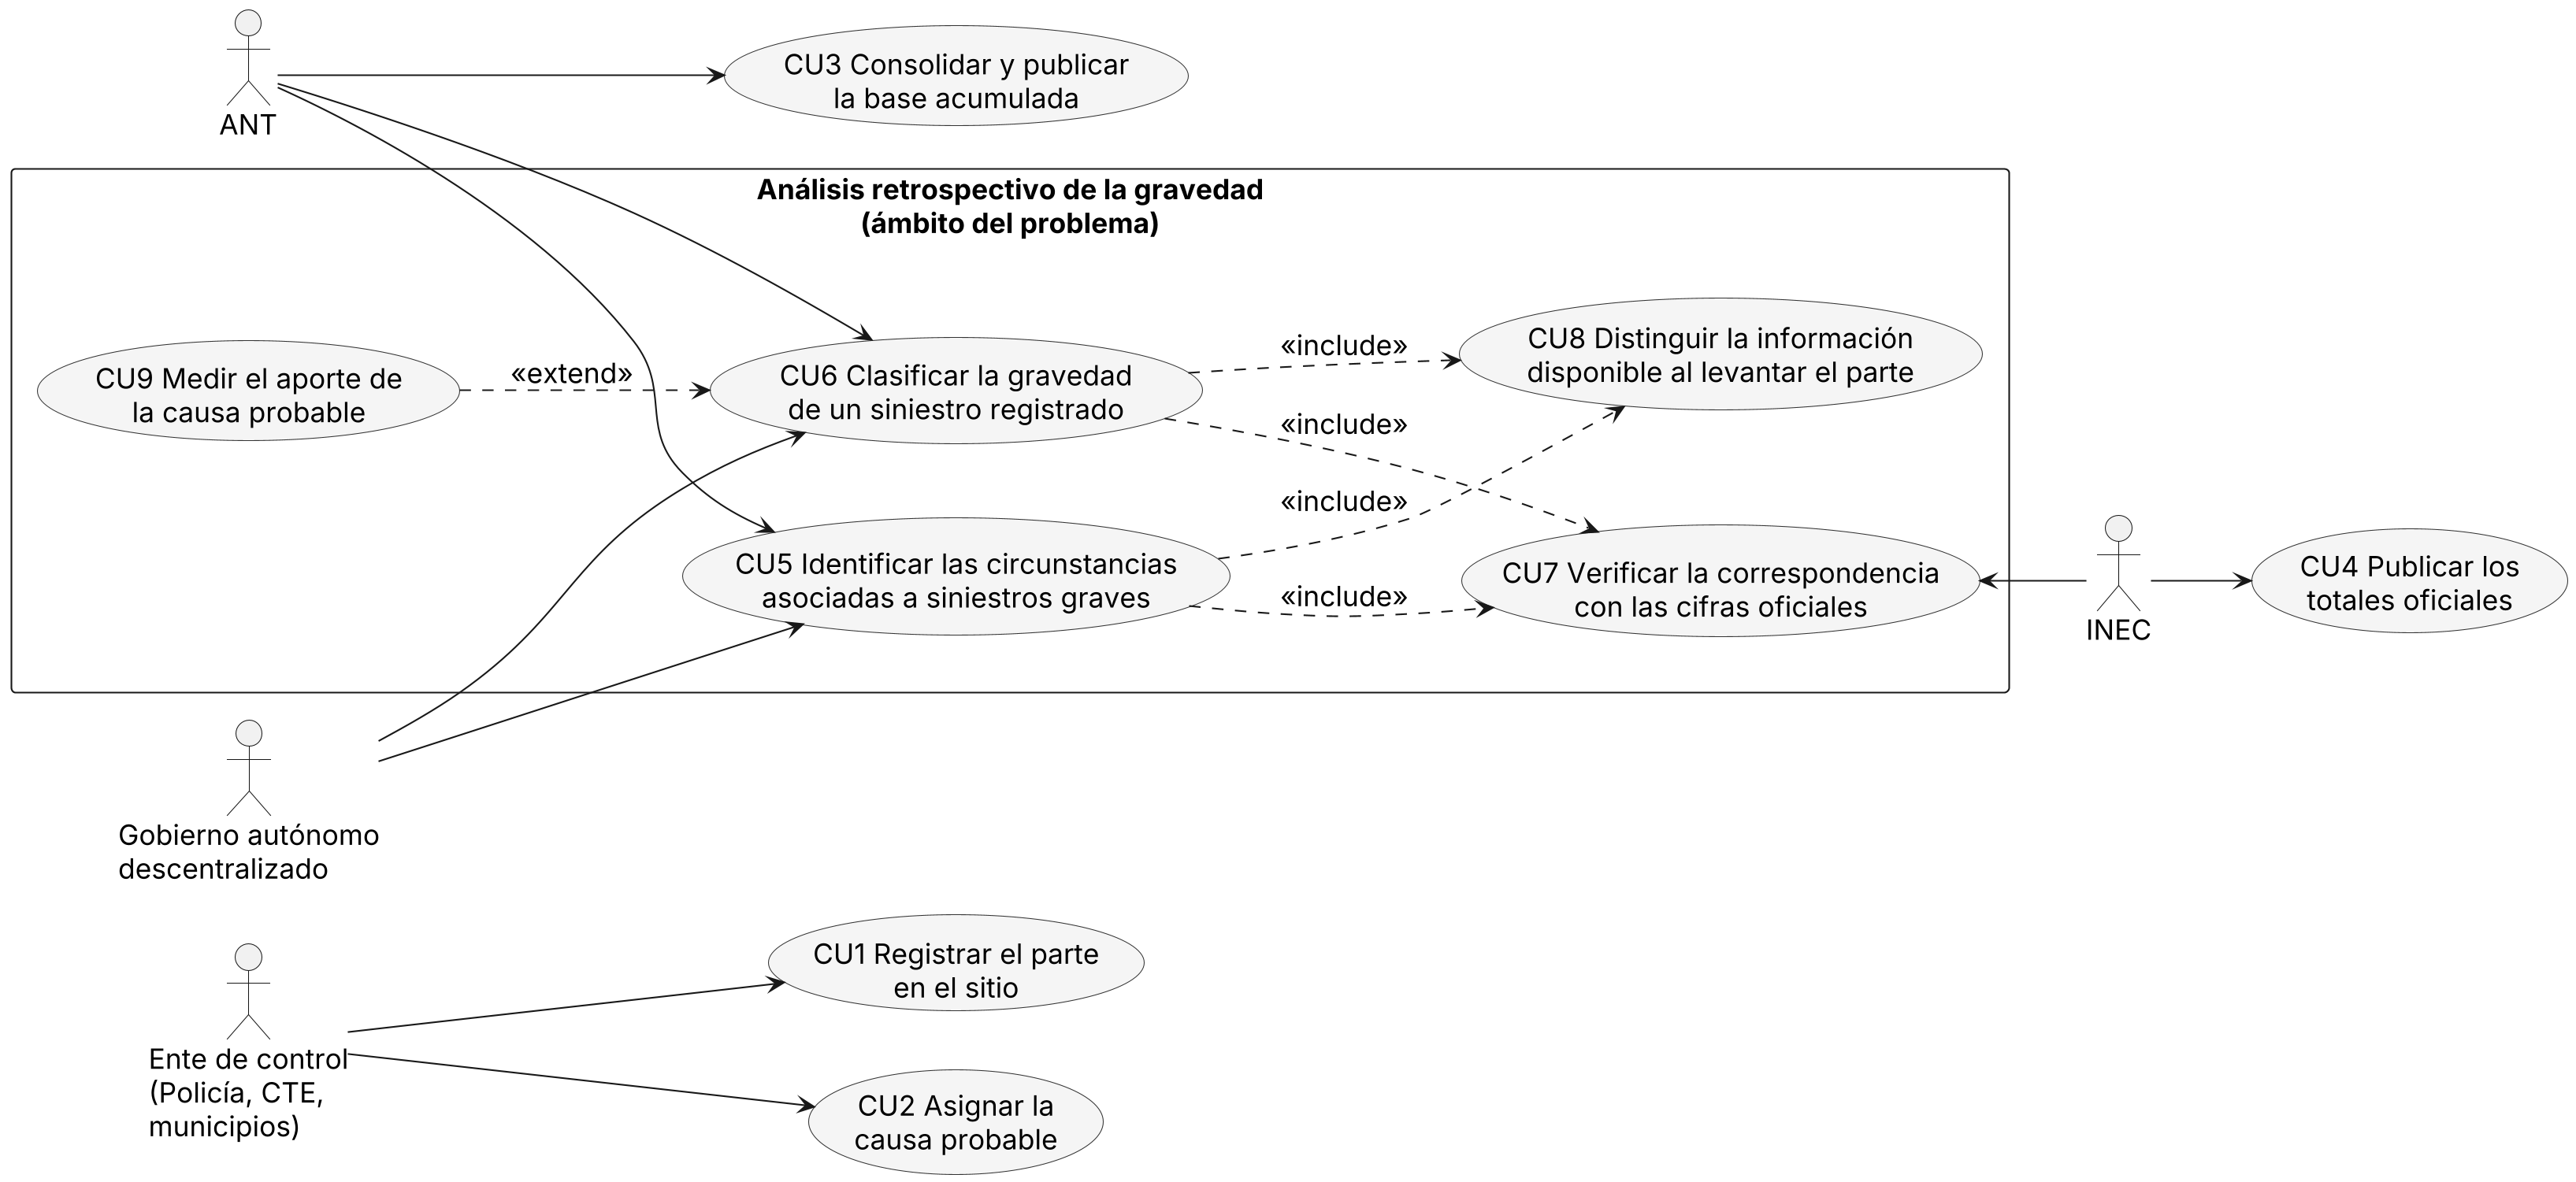
\includegraphics[width=1.10\textwidth]{figuras/M1_casos_de_uso.png}}
\caption{M1. Casos de uso del análisis retrospectivo de la gravedad.}
\label{fig:m1}
\end{figure}

\paragraph{M2. Clases de dominio: qué datos existen y qué papel cumple cada uno.} \texttt{Siniestro} se relaciona uno a uno con \texttt{Ubicación} y con \texttt{CircunstanciaDelEvento}, y uno a muchos con \texttt{VehiculoInvolucrado}; cada siniestro pertenece a un \texttt{EnteDeControl}. Esas cuatro clases forman el conjunto~A. \texttt{CausaProbable} se asocia con cero o una por siniestro y forma el conjunto~B, porque se asigna al investigar. \texttt{Participante}, de uno a 43 por siniestro, queda excluida: su atributo \texttt{condicion} contiene el valor \texttt{fallecido}. De los participantes se deriva \texttt{Resultado}, y de este la \texttt{Etiqueta}; ambos son el desenlace y nunca son entrada. Las coordenadas, la dirección y el nombre de la vía también se excluyen por privacidad. Los estereotipos de la figura indican el papel de cada clase.

\begin{figure}[htbp]
\centering
\makebox[\textwidth][c]{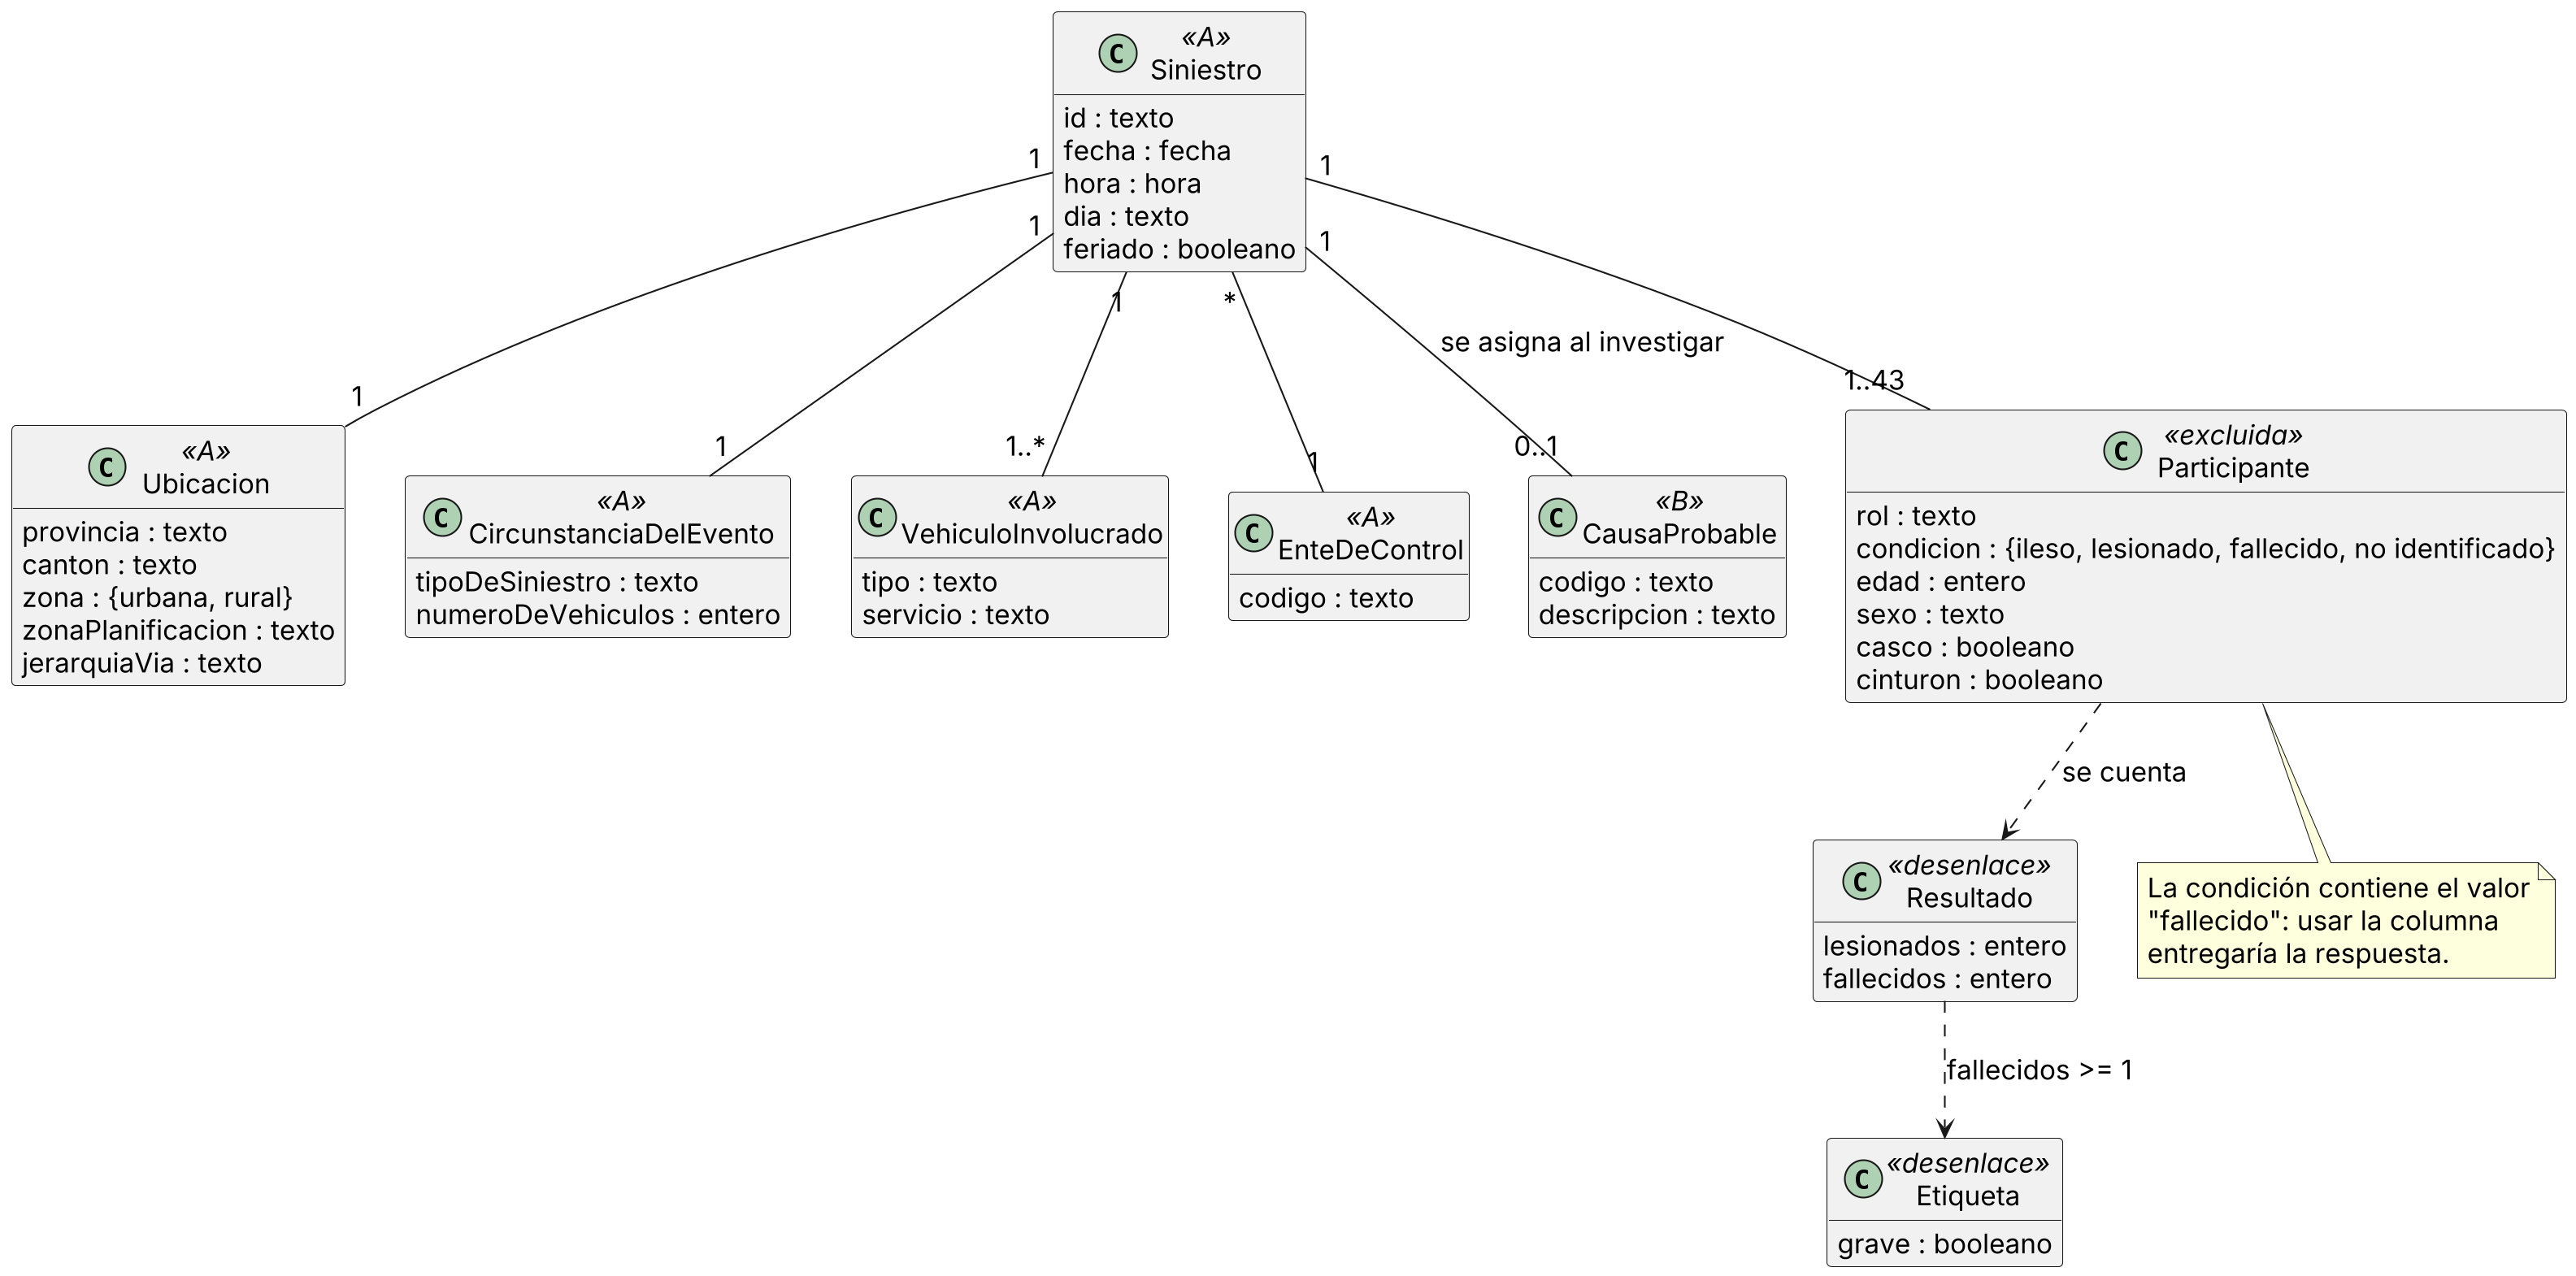
\includegraphics[width=1.08\textwidth]{figuras/M2_clases_de_dominio.png}}
\caption{M2. Clases del dominio del problema y clasificación de sus atributos.}
\label{fig:m2}
\end{figure}

\paragraph{M3. Actividad: cómo se produce y se usa el dato.} El diagrama tiene cuatro carriles. El ente de control atiende el siniestro y levanta el parte con las circunstancias del conjunto~A; si no puede determinar un campo, lo registra como \texttt{ND} o no identificado. Luego registra a los participantes y su condición, que constituye el desenlace; si una persona fallece después del evento, sigue registrada como lesionada según la convención de la sección~2.2. Al terminar la investigación asigna la causa probable, que forma el conjunto~B, y envía el parte a la ANT. Esta consolida los partes de los 16 entes de control y publica el archivo acumulado del año, que conserva los defectos de origen descritos en la Tabla~\ref{tab:a3}. El INEC procesa los mismos registros y publica totales trimestrales. El gobierno autónomo descentralizado consulta ambas fuentes, pero los totales no responden qué circunstancias se asocian con los fallecidos en sitio; esa necesidad no cubierta es el problema que se analiza.

\begin{figure}[htbp]
\centering
\makebox[\textwidth][c]{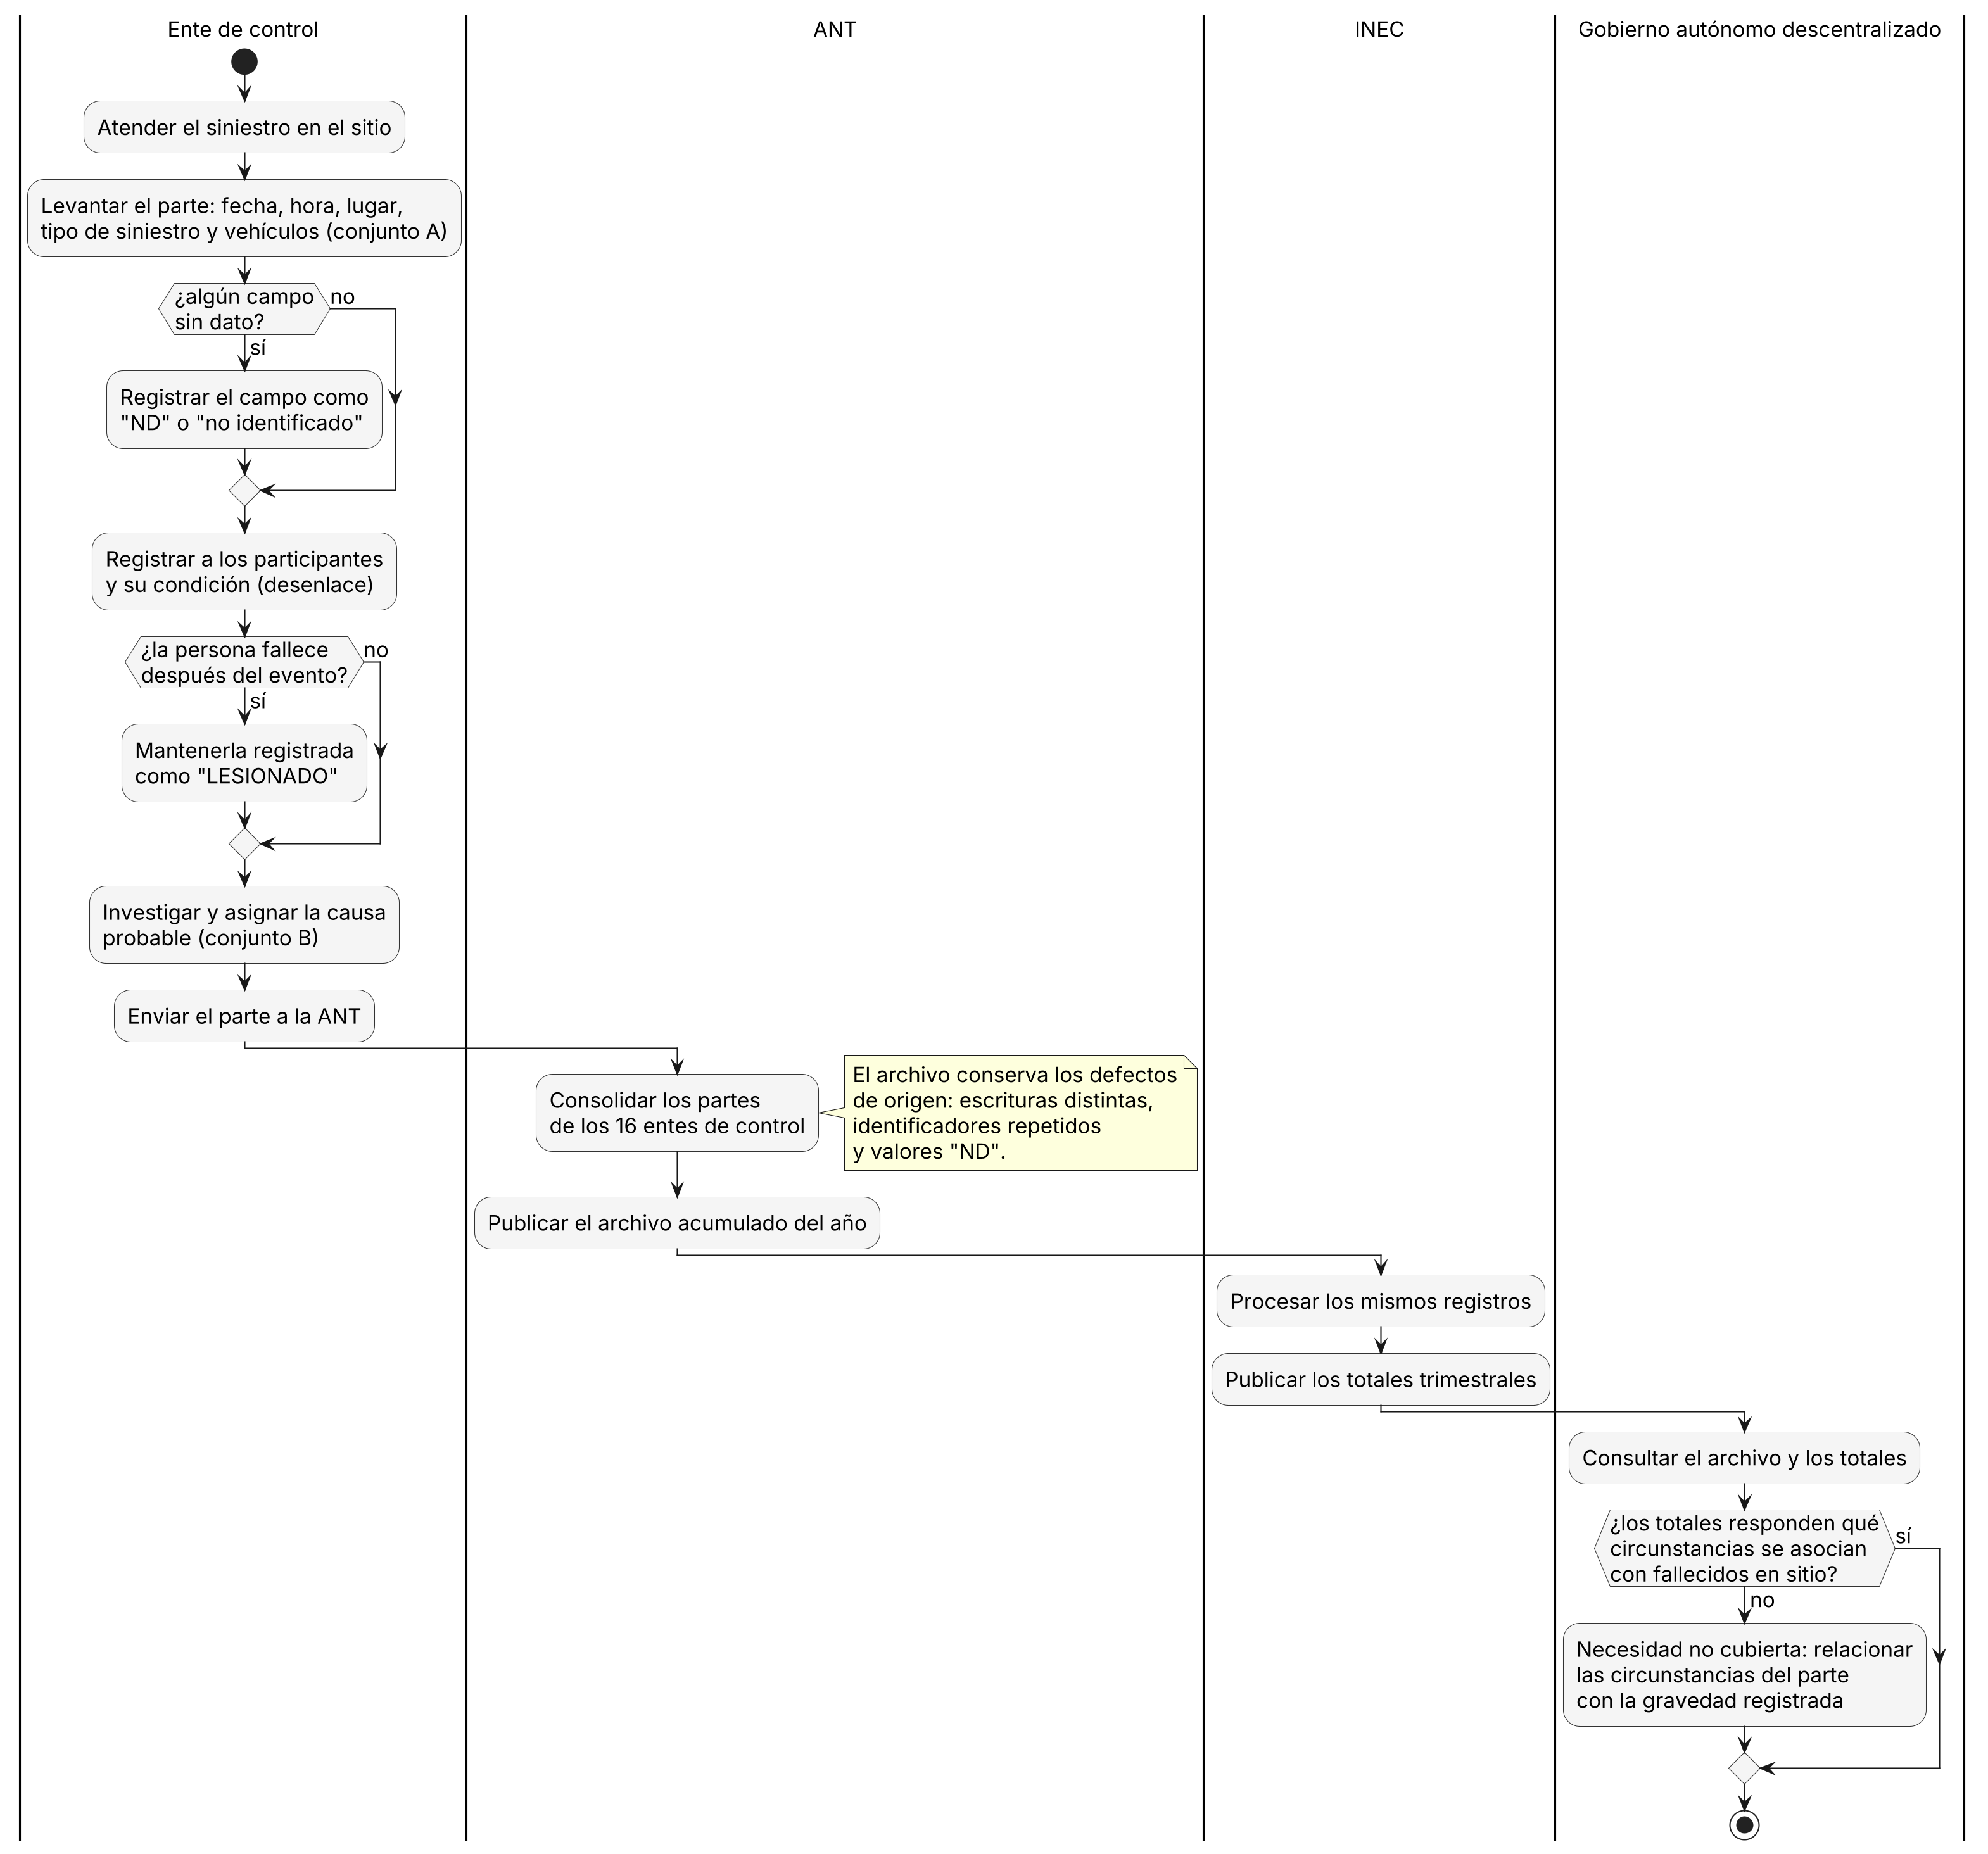
\includegraphics[width=1.10\textwidth,height=0.80\textheight,keepaspectratio]{figuras/M3_actividad.png}}
\caption{M3. Producción, consolidación y uso del dato del siniestro.}
\label{fig:m3}
\end{figure}

\paragraph{M4. Estados: cuándo existe cada información.} Un siniestro ocurre, es atendido en el sitio y llega al estado \emph{parte levantado}, en el que se conocen la fecha, la hora, el lugar, el tipo de siniestro y los vehículos. Después pasa a \emph{causa asignada}, luego a \emph{consolidado por la ANT} y finalmente a \emph{publicado con corte al 30 de septiembre de 2026}. El instante del análisis retrospectivo es \emph{parte levantado}. El recuento de víctimas existe ya en ese estado, pero no puede usarse como entrada porque es lo que se quiere clasificar.

\begin{figure}[htbp]
\centering
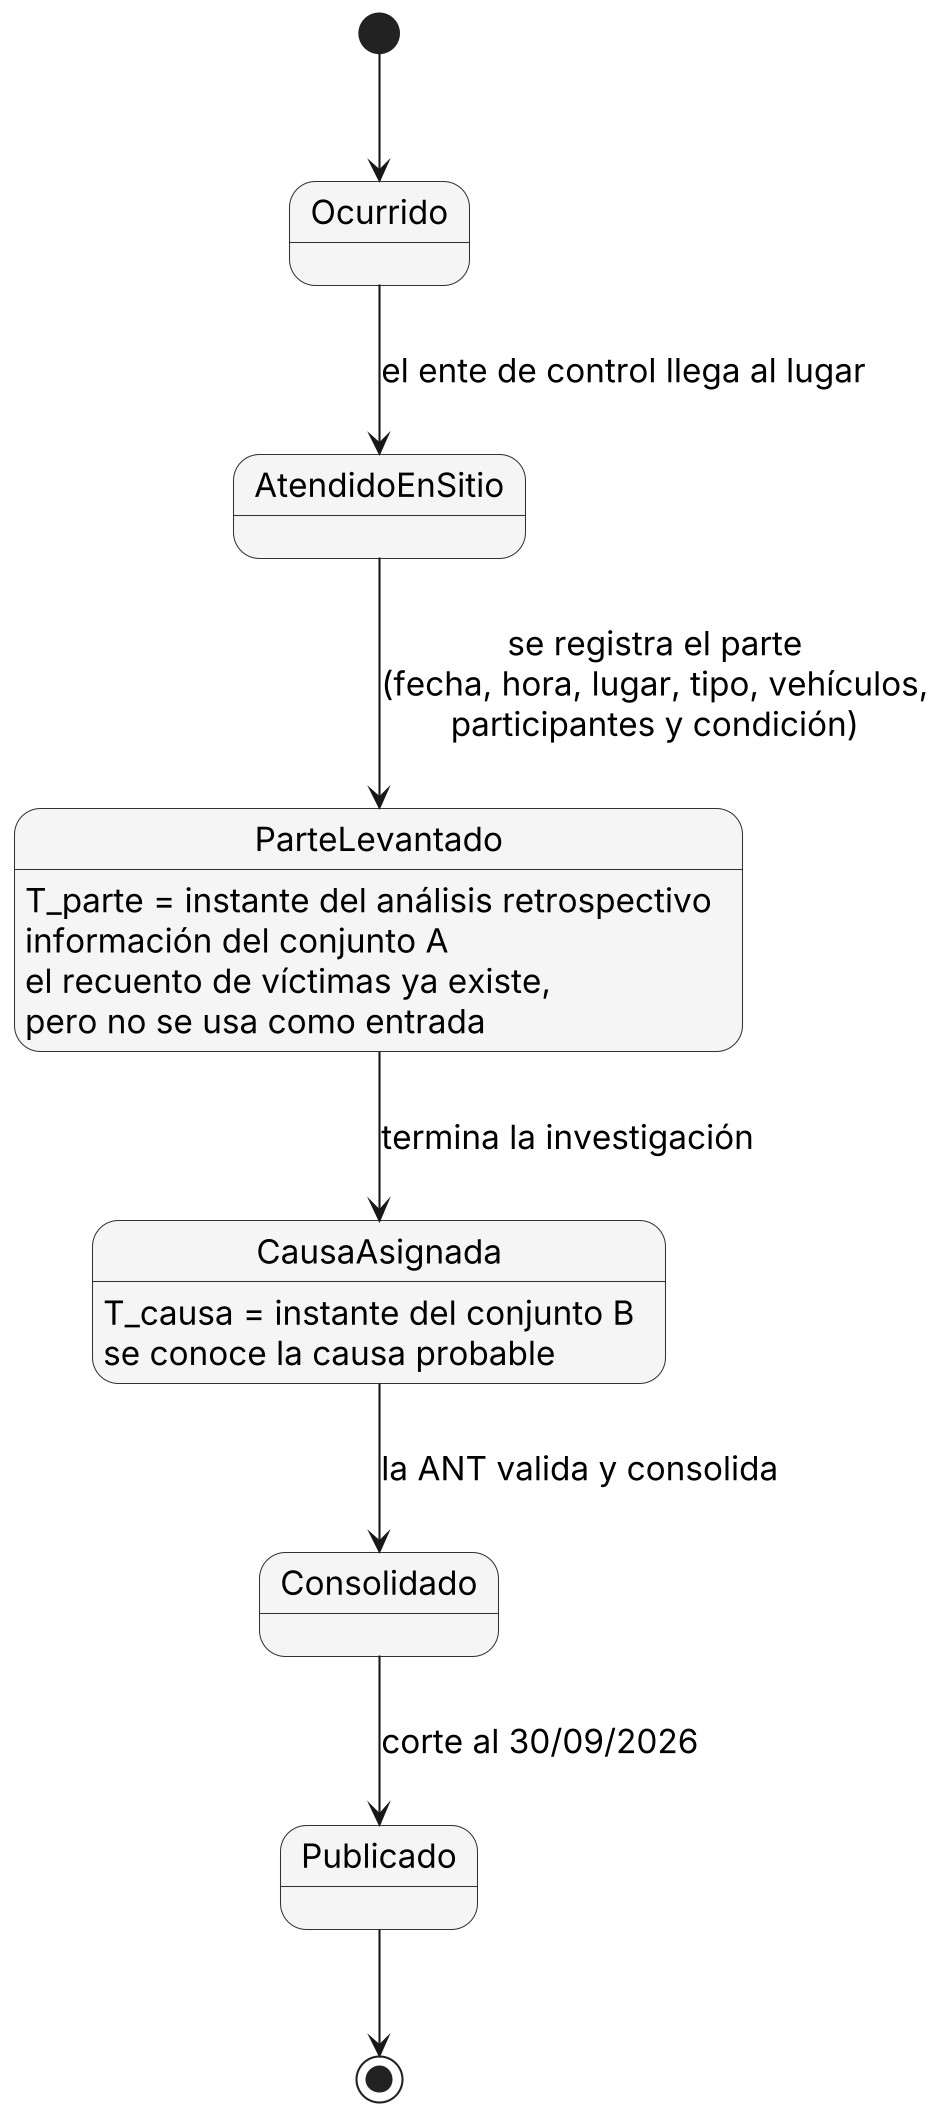
\includegraphics[width=0.92\textwidth,height=0.62\textheight,keepaspectratio]{figuras/M4_estados.png}
\caption{M4. Estados del registro e información disponible en cada uno.}
\label{fig:m4}
\end{figure}


\paragraph{M5. Secuencia: cómo circula la información.} El ente de control envía a la ANT el parte con las circunstancias y la condición de los participantes, y más tarde la causa probable. Si una persona fallece después del evento, el registro no cambia y la persona sigue como lesionada. La ANT consolida los partes, entrega los registros al INEC y publica el archivo acumulado; el INEC publica los totales trimestrales. Con ambas fuentes, el gobierno autónomo descentralizado busca qué circunstancias se asocian con los fallecidos en sitio, y en los territorios con menos de 30 siniestros la proporción local no es confiable. La secuencia termina en la misma necesidad que M3: el archivo contiene el desenlace, pero no la relación entre circunstancias y gravedad.

\begin{figure}[htbp]
\centering
\makebox[\textwidth][c]{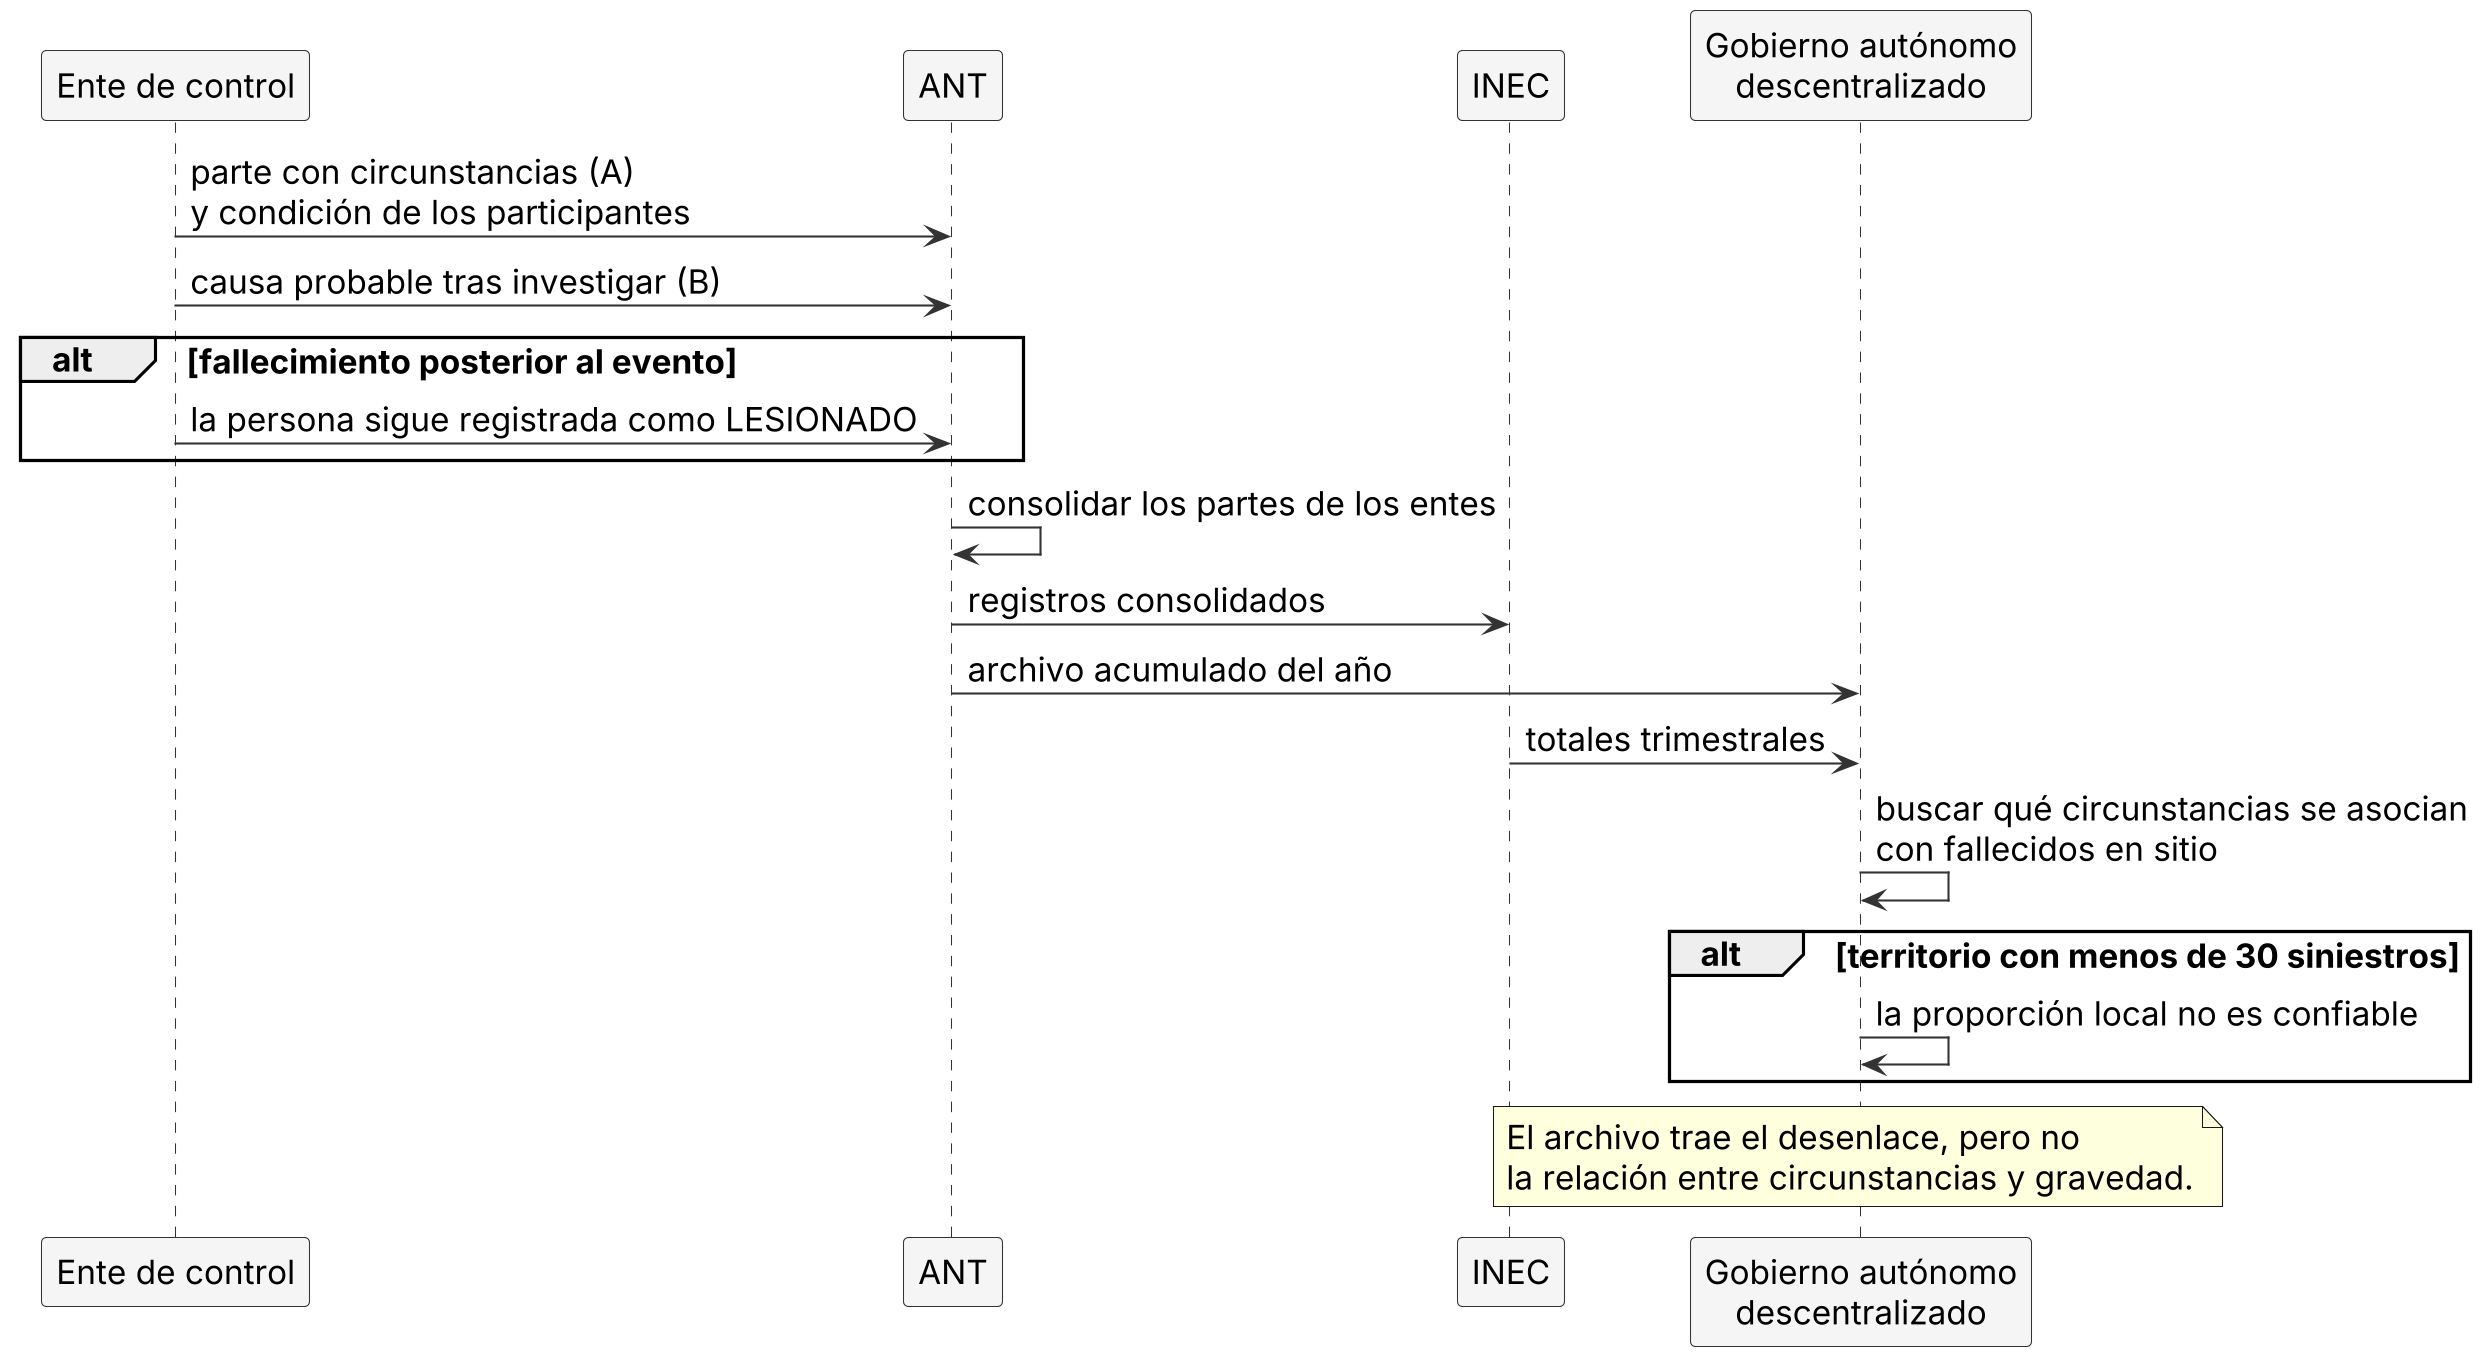
\includegraphics[width=1.05\textwidth]{figuras/M5_secuencia.png}}
\caption{M5. Secuencia de mensajes entre los actores.}
\label{fig:m5}
\end{figure}

\subsection{Escenarios de los casos de uso}
\label{sec:escenarios}

Cada caso de uso de M1 se describe con un escenario principal y uno alterno o de excepción tomado del archivo real, con las mismas excepciones que M3. CU1 a CU4 quedan fuera del límite del análisis, pero se describen porque producen el dato del que dependen los demás; CU7 y CU8 no tienen actor directo porque los incluyen CU5 y CU6, y CU9 se activa desde CU6.

\newcommand{\escenario}[7]{%
\begin{table}[H]
\centering
\small
\caption{#1}
\begin{tabularx}{\textwidth}{>{\raggedright\arraybackslash\bfseries}p{2.9cm}X}
\toprule
Actor & #2 \\
Objetivo & #3 \\
Precondición & #4 \\
\midrule
Escenario 1 (principal) & #5 \\
Escenario 2 (alterno) & #6 \\
\midrule
Postcondición & #7 \\
\bottomrule
\end{tabularx}
\end{table}}

\escenario{CU1. Registrar el parte en el sitio}
{Ente de control (Policía Nacional, CTE, entidades municipales).}
{Dejar constancia del siniestro con sus circunstancias, vehículos, participantes y condición.}
{Ocurrió un siniestro y el ente de control lo atiende en el sitio.}
{(1) El ente atiende el siniestro. (2) Registra fecha, hora, lugar, tipo de siniestro y vehículos. (3) Registra a los participantes y su condición. (4) Envía el parte a la ANT.}
{\emph{Campo sin dato o fallecimiento posterior.} Si no puede determinar un campo, como la jerarquía de la vía o el tipo de vehículo, lo registra como \texttt{ND} o no identificado. Si una persona fallece después del evento, en la CTE sigue registrada como \texttt{LESIONADO}.}
{El siniestro queda registrado y el recuento de víctimas ya está definido.}

\escenario{CU2. Asignar la causa probable}
{Ente de control.}
{Determinar la causa más probable del siniestro una vez investigado el hecho.}
{El parte fue levantado (CU1).}
{(1) El ente investiga el hecho. (2) Asigna una de las 26 causas probables del catálogo de la ANT. (3) Completa el parte con el código y la descripción de la causa.}
{\emph{Causa que refleja el desenlace.} La causa se asigna cuando ya se conoce lo ocurrido, por ejemplo un peatón que cruza sin respetar la señalización. Por eso la causa no forma parte del conjunto~A y se trata por separado en el conjunto~B.}
{El siniestro tiene una causa asignada, posterior al levantamiento del parte.}

\escenario{CU3. Consolidar y publicar la base acumulada}
{ANT.}
{Unir los partes de los entes de control y publicar el archivo acumulado del año.}
{La ANT recibió los partes del periodo.}
{(1) La ANT recibe los partes de los 16 entes de control. (2) Los consolida. (3) Publica el archivo acumulado con corte al 30 de septiembre de 2026.}
{\emph{Republicación del acumulado.} Cada mes el archivo se publica de nuevo con todos los meses anteriores y puede incluir registros añadidos o corregidos. Por eso cada copia se identifica por su fecha de descarga (H-06).}
{El archivo está disponible con sus defectos de origen (Tabla~\ref{tab:a3}).}

\escenario{CU4. Publicar los totales oficiales}
{INEC.}
{Publicar las cifras oficiales de siniestros, lesionados y fallecidos por trimestre.}
{El INEC recibió los registros consolidados de la ANT.}
{(1) El INEC procesa los registros. (2) Publica los totales del primer trimestre de 2026: 4.789 siniestros, 4.032 lesionados y 603 fallecidos \cite{ref1}.}
{\emph{Periodo sin boletín.} Si el periodo que se quiere verificar no tiene boletín trimestral, se usa otra cifra oficial del mismo periodo, como la de la ANT para enero a mayo: 8.718 siniestros \cite{ref7}.}
{Existen totales oficiales con los que puede verificarse el archivo.}

\escenario{CU5. Identificar las circunstancias asociadas a siniestros graves}
{ANT y gobiernos autónomos descentralizados; entes de control como lectores.}
{Conocer cómo varía la proporción de siniestros graves entre grupos definidos con el conjunto~A (OE1).}
{El archivo fue verificado (CU7) y la información disponible está delimitada (CU8).}
{(1) Se agrupan los siniestros por una circunstancia del conjunto~A, por ejemplo el tipo de siniestro. (2) Para cada grupo se obtienen el número de casos, la proporción de graves y una medida de incertidumbre. (3) Los grupos se ordenan: van del 3,0\,\% en colisiones al 45,8\,\% en arrollamientos.}
{\emph{Grupo o territorio con pocos casos.} Si un grupo, como un cantón o una causa poco frecuente, tiene menos de 30 casos, su proporción es inestable y no se reporta como de mayor gravedad.}
{Las diferencias entre grupos quedan descritas como asociaciones, con su número de casos e incertidumbre.}

\escenario{CU6. Clasificar la gravedad de un siniestro registrado}
{ANT y gobiernos autónomos descentralizados.}
{Determinar si un siniestro ya registrado tuvo al menos un fallecido en sitio, usando solo las circunstancias del parte (OE2).}
{El archivo fue verificado (CU7) y la información disponible está delimitada (CU8).}
{(1) Se toma un siniestro ya registrado. (2) Se usan solo sus variables del conjunto~A. (3) Se obtiene la probabilidad de que registre al menos un fallecido en sitio. (4) La clasificación se compara con las dos referencias sencillas en casos posteriores en el tiempo.}
{\emph{Siniestro con información incompleta.} Si el parte tiene campos en \texttt{ND}, como ocurre con la jerarquía de la vía en el 66,4\,\% de los registros, ese valor se trata como una categoría propia y la clasificación se apoya en el resto de las circunstancias.}
{El siniestro queda clasificado de forma retrospectiva, sin anticipar siniestros futuros.}

\escenario{CU7. Verificar la correspondencia con las cifras oficiales}
{Sin actor directo; lo incluyen CU5 y CU6. El INEC aporta los totales.}
{Comprobar que el archivo corresponde a la fuente oficial (CA-01).}
{Existen una copia del archivo con fecha de descarga y totales oficiales de un periodo común (CU4).}
{(1) Se cuentan siniestros, lesionados y fallecidos del primer trimestre en el archivo: 4.789, 4.032 y 603. (2) Se comparan con los del INEC. (3) La diferencia es del 0\,\% y el archivo se considera válido.}
{\emph{Diferencia mayor al 1\,\%.} Si algún total difiere en más del 1\,\%, la diferencia y su posible explicación, como una republicación del acumulado, se documentan antes de interpretar cualquier resultado.}
{La correspondencia del archivo con las cifras oficiales queda documentada.}

\escenario{CU8. Distinguir la información disponible al levantar el parte}
{Sin actor directo; lo incluyen CU5 y CU6.}
{Separar lo que existe al levantar el parte de lo que aparece después o contiene el desenlace (CA-02).}
{Se conoce el catálogo de las 374 columnas del archivo.}
{(1) Las circunstancias del evento forman el conjunto~A. (2) La causa probable se separa en el conjunto~B. (3) \texttt{FALLECIDOS} y \texttt{LESIONADOS} se tratan como desenlace. (4) \texttt{CONDICION\_1} a \texttt{CONDICION\_43} se excluyen porque coinciden con el recuento de víctimas en el 100\,\% de los registros. (5) Los campos personales y de ubicación exacta se excluyen.}
{\emph{Valores inconsistentes o identificador repetido.} Diez registros escriben \texttt{colisión} en minúscula, 14 tienen valor~0 en la jerarquía de la vía y un identificador aparece en dos siniestros de fechas distintas. Las escrituras se unifican, el 0 se agrupa con \texttt{ND} y ambas filas del identificador repetido se conservan sin usarlo como llave.}
{Cada variable tiene un papel definido: entrada de A, entrada de B, desenlace o excluida.}

\escenario{CU9. Medir el aporte de la causa probable}
{Sin actor directo; extiende a CU6.}
{Cuantificar cuánto añade la causa probable a la clasificación y con qué riesgo.}
{Existe la clasificación con el conjunto~A (CU6).}
{(1) A las circunstancias del conjunto~A se agrega la causa probable. (2) Con los mismos siniestros y el mismo orden temporal, se compara cuánto permite distinguir cada conjunto los siniestros graves. (3) La diferencia se reporta como aporte de la causa.}
{\emph{Mejora muy grande con el conjunto~B.} Si B supera ampliamente a A, la mejora se interpreta con cautela, porque la causa puede reflejar el desenlace, y el conjunto~A se mantiene como escenario principal.}
{El aporte de la causa probable queda medido y separado del escenario principal.}

\subsection{Matrices de trazabilidad}
\label{sec:trazabilidad}

La primera matriz relaciona cada objetivo con los requerimientos de la sección~7, los datos de la sección~6, los actores de la sección~4, las restricciones de la sección~8, los criterios de la sección~9 y los modelos de esta sección. Las celdas con varios identificadores indican que un mismo elemento interviene en más de un objetivo.

\begin{longtable}{p{1.3cm}p{2.7cm}p{2.0cm}p{2.0cm}p{1.6cm}p{1.8cm}p{1.8cm}}
\caption{Trazabilidad entre objetivos, requerimientos, datos, actores, restricciones, criterios y modelos}
\label{tab:trazabilidad}\\
\toprule
Obj. & Requerimientos & Datos & Actores & Restr. & Criterios & Modelos \\
\midrule
\endfirsthead
\multicolumn{7}{l}{\footnotesize\itshape (continuación)}\\
\toprule
Obj. & Requerimientos & Datos & Actores & Restr. & Criterios & Modelos \\
\midrule
\endhead
\bottomrule
\endfoot
General & RF-01, RF-02, RF-03, RNF-01 & Archivo de la ANT completo & ANT, INEC & R-04, R-05, R-10 & CA-01, CA-08 & M1 (CU7), M3, M5 \\
OE1 & RF-04, RF-05, RF-10, RNF-03, RNF-05 & Conjunto A y etiqueta & ANT, entes y gobiernos locales & R-04, R-07, R-08 & CA-03 & M1 (CU5), M2, M3 \\
OE2 & RF-03, RF-06, RF-07, RF-08, RF-09, RNF-01, RNF-02, RNF-04 & Conjuntos A y B y etiqueta & ANT, gobiernos locales & R-01, R-02, R-03, R-06 & CA-02, CA-04 a CA-07 & M1 (CU6, CU8, CU9), M2, M4 \\
OE3 & RF-11, RNF-04 & Resultados del modelo seleccionado & ANT, gobiernos locales & R-01, R-08, R-09 & CA-09 & M1 (CU6) \\
\end{longtable}

La segunda matriz desagrega la anterior por requerimiento: cada fila indica el caso de uso que lo origina, el dato que lo alimenta, el actor del que depende, el criterio que lo comprueba y el modelo donde aparece.

\begin{longtable}{p{1.3cm}p{1.7cm}p{3.6cm}p{2.3cm}p{2.1cm}p{1.8cm}}
\caption{Trazabilidad por requerimiento}
\label{tab:trazabilidad-rf}\\
\toprule
Req. & CU & Dato & Actor & Criterio & Modelo \\
\midrule
\endfirsthead
\multicolumn{6}{l}{\footnotesize\itshape (continuación)}\\
\toprule
Req. & CU & Dato & Actor & Criterio & Modelo \\
\midrule
\endhead
\bottomrule
\endfoot
RF-01 & CU7 & Totales del primer trimestre del archivo y del INEC & ANT, INEC & CA-01 & M1, M5 \\
RF-02 & CU6, CU8 & \texttt{FALLECIDOS} & ANT por la convención de registro & CA-01, CA-08 & M2, M4 \\
RF-03 & CU8 & \texttt{CONDICION\_k}, \texttt{FALLECIDOS}, \texttt{LESIONADOS} & Entes de control & CA-02 & M2, M4 \\
RF-04 & CU8 & Jerarquía de la vía, tipo de vehículo, tipo de siniestro (Tabla~\ref{tab:a3}) & Entes de control & CA-02, CA-03 & M3 \\
RF-05 & CU5 & Conjunto A y etiqueta & ANT, gobiernos locales & CA-03 & M1, M5 \\
RF-06 & CU6 & \texttt{FECHA} y etiqueta & ANT, gobiernos locales & CA-05, CA-07 & M4 \\
RF-07 & CU6, CU9 & Conjuntos A y B & ANT, gobiernos locales & CA-04 & M1, M2 \\
RF-08 & CU6 & Etiqueta de la prueba (ago--sep) & ANT, gobiernos locales & CA-04, CA-05 & M1 \\
RF-09 & CU6 & Probabilidades y etiqueta & ANT, gobiernos locales & CA-06 & M1 \\
RF-10 & CU5, CU6 & Resultados de OE1 y OE2 & ANT, gobiernos locales & CA-03, CA-08 & M1, M5 \\
RF-11 & CU6 & Modelo seleccionado & ANT, gobiernos locales & CA-09 & M1 \\
RNF-01 & CU7 & Copia del archivo con fecha de descarga & ANT & CA-01, CA-09 & M3 \\
RNF-02 & CU6 & Tramos temporales (Tabla~\ref{tab:a6}) & ANT, gobiernos locales & CA-04, CA-06 & M4 \\
RNF-03 & CU8 & Defectos de la Tabla~\ref{tab:a3} & Entes de control & CA-02 & M3 \\
RNF-04 & CU5, CU6 & Resultados & Gobiernos locales & CA-08 & M1 \\
RNF-05 & CU5, CU6 & Resultados agregados & Gobiernos locales & CA-03 & M5 \\
\end{longtable}
